\subsection{Powering the Display}
\begin{figure*}
\onecolumn
\setcounter{problem}{6}  
\input{./chapter1/tables/arduinoport}
%
\setcounter{problem}{0}  
\twocolumn
\end{figure*}

%
\begin{problem}
	Plug the display to the breadboard shown in Fig. \ref{fig_1_1}. The breadboard can be divided into 5 segments.  In each of the green segements, the pins are internally connected so as to have the same voltage.  Similarly, in the central segments, the pins in each column  are internally connected in the same fashion as the blue columns. 
%
\end{problem}
%
\begin{figure}[!ht]
\begin{center}
\includegraphics[width=\columnwidth]{./chapter1/figs/breadboard}
\end{center}
\captionof{figure}{Breadboard}
\label{fig_1_1}	
\end{figure}
%
\begin{problem}
	Connect one end of the 220 $\Omega$ resistor to the COM pin of the display in Fig. \ref{fig_1_2} and the other end to an extreme pin of the breadboard.	The seven segment display has eight pins, $a, b, c, d, e, f, g$ and $dot$ that take an active LOW input, i.e.  the LED will glow only if the input is connected to ground.  Each of these pins is connected to an LED segment.  The $dot$ pin is  reserved for the $\cdot$ LED.  
%
\end{problem}
%
\begin{figure}
\begin{center}
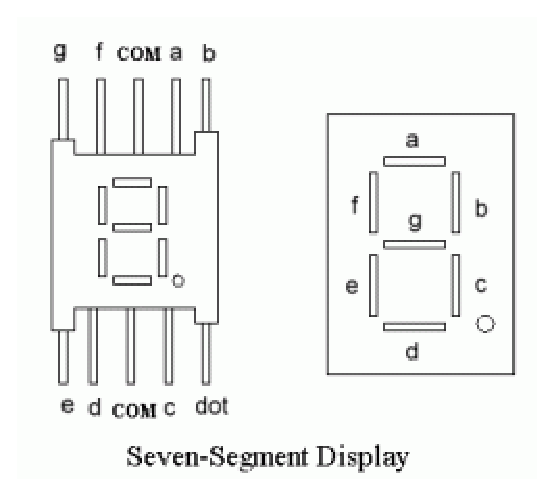
\includegraphics[width=\columnwidth]{./chapter1/figs/sevenseg}
\end{center}
\captionof{figure}{Seven Segment Display. }
\label{fig_1_2}
\end{figure}	%%
\begin{problem}
	Connect the 3.3$V$ pin of the Pi shown in Figs. \ref{fig_1_3a} and  \ref{fig_1_3b}  to an  extreme pin that is in the same segment as the 220 $\Omega$ resistor pin. 
\end{problem}	
\renewcommand{\thefigure}{\theproblem.\arabic{figure}}
\begin{figure}[!ht]
\begin{center}
\includegraphics[width=\columnwidth]{./chapter1/figs/gpio2}
\end{center}
\captionof{figure}{GPIO pin snapshot on Pi \cite{gpio_pins}.}
\label{fig_1_3a}	
\end{figure}
%
\begin{figure}
\begin{center}
\includegraphics[width=\columnwidth]{./chapter1/figs/gpio1}
\end{center}
\captionof{figure}{GPIO Wiring Pi \cite{wiringpi} pin configuration.}
\label{fig_1_3b}	
\end{figure}
\renewcommand{\thefigure}{\theproblem}
%
\begin{problem}
	Connect the GND pin of the Pi to the opposite extreme pin of the breadboard
\end{problem}
\begin{problem}
	Connect the {\em dot} pin of the display to a pin in the same segment as the GND pin.  What do you observe?
\end{problem}
\subsection{Controlling the Display}
\begin{problem}
	Generate the number 1 on the display by connecting the pins $a-g$ to GND according to Table \ref{table_1_6}.
	\end{problem}
%
\begin{problem}
	Complete Table \ref{table_1_6} for all numbers between 0-9.
\end{problem}
%
\begin{problem}
	Now generate the numbers from 0-9 on the display using Table \ref{table_1_6}.
\end{problem}
%
\begin{problem}
	Connect the 7447 IC decoder $\bar{a}-\bar{g}$ pins  in Fig. \ref{fig_1_9} to the $a-g$ pins of the display respectively.
\end{problem}
%
\begin{figure}[!ht]
\begin{center}
\includegraphics[width=\columnwidth]{./chapter1/figs/7447IC}
\end{center}
\captionof{figure}{7447 to seven segment display decoder.}
\label{fig_1_9}	
\end{figure}
%

\begin{problem}
	Connect the $V_{cc}$ and GND pins of the decoder in to the  supply and GND pins of the breadboard.
\end{problem}
\begin{problem}
	Connect the A,B,C,D pins in Fig. \ref{fig_1_9}  to pins in the GND extreme segment of the breadboard.  What do you observe?
\end{problem}
\begin{problem}
	Now remove the D pin from the breadboard and observe the display output.
\end{problem}
\begin{problem}
	Generate a table with A,B,C,D inputs and the equivalent decimal number output.
\end{problem}
The 7447 IC helps in displaying decimal numbers on the seven segment display.  The $\bar{a}-\bar{f}$, pins of the 7447 IC are connected to the $a-f$ pins of the display. $V_cc$ should be connected to a 5V power source. The input pins of the decoder are A,B,C and D, with A being the lowest significant bit (LSB) and D being the most significant bit (MSB).  For example, the number 5 is visible on the display when the A,B,C and D inputs are the following.
\begin{center}
	\begin{tabular}{|c|c|c|c|c|}
\hline
D & C & B & A & Decimal
\\ \hline
0 & 1 & 0 & 1 & 5
\\
\hline
\end{tabular}
\end{center}
